\documentclass[12pt, a4paper, onecolumn]{report}  
  \usepackage[english, brazilian, portuguese]{babel}
  \usepackage[T1]{fontenc}
  \usepackage{ae}
  \usepackage[utf8]{inputenc}
  \usepackage{graphicx, subfig}
  \usepackage{algorithm, algorithmic}
  \usepackage{amsmath}
  \usepackage{amsthm}
  \usepackage{listings}  
  \graphicspath{{images//}}

\begin{document} 

\begin{titlepage}

\begin{minipage}{0.2\linewidth}
 
\includegraphics[width=0.8\textwidth]{minerva.jpg}
\end{minipage}
\begin{minipage}{0.8\linewidth}
 \textbf{Universidade Federal do Rio de Janeiro}\\
 Departamento de Ciência da Computação\\
\end{minipage}

\begin{center}
\vspace{2cm}
\Large
\textbf{Trabalho de Simulação}
\vspace{0.5cm}
\normalsize
\end{center}
\vfill

\begin{flushright}
Autores:

\vspace{0.125cm}

Marco Vinícius Lima Reina de Barros

\vspace{0.25cm}

Pedro Henrique Pereira de Jesus

\vspace{0.25cm}

Ronald Andreu Kaiser
\end{flushright}
\vspace{0.70cm}
\begin{center}
Todos os membros do grupo participaram da implementação do código e da documentação do relatório.

\vspace{0.25cm}

\today
\end{center}

\vspace{2cm}

\end{titlepage}

\tableofcontents
\chapter{Introdução}
\section{Funcionamento geral}

O simulador possui uma lista de eventos que é processada continuamente, até alcançar um número máximo de clientes que desejamos atender por rodada.

São executadas tantas rodadas quanto forem necessárias até todos os intervalos de confiança dos valores que estão sendo estimados forem válidos, ou seja, $<=10\%$ da média do estimador.

Inicialmente, calculamos o tempo de chegada do primeiro cliente que representa um evento de chegada no sistema. A passsagem de um cliente pelo sistema possibilita a criação dos seguintes eventos:
\begin{itemize}
\item <tempo, tipo: chegada no sistema>
\item <tempo, tipo: entrada no servidor pela primeira vez>
\item <tempo, tipo: saída do servidor>
\item <tempo, tipo: entrada no servidor pela segunda vez>
\end{itemize}

Quando um evento de chegada ocorre, outro evento de chegada é criado com o tempo definido com o tempo de chegada baseado em uma distribuição exponencial, que representa o tempo de chegada do próximo cliente. Deste modo, os clientes vão chegando no sistema e a lista de eventos é processada.

Quando um evento é processado, ele é removido da lista de eventos e os novos eventos gerados a partir deste são criados e adicionados na lista, ordenada pelos tempos em que cada evento ocorre.

Todos os parâmetros, descritos na seção \ref{sec:parametros} são passados para o simulador em sua inicialização.

\section{Estruturas internas utilizadas}
Para viabilizar a implementação da ideia geral apresentada acima, dividimos o simulador em alguns módulos, abaixo estão explicitados os mais importantes:\\

\textbf{Módulos utilitários:}

\begin{itemize}
  \item Estimator: Módulo que possui métodos para retornar os estimadores de média, variância e calcula intervalos de confiança.
  \item Dist: Módulo com o método que retorna os tempos aleatórios de chegada de uma distribuição exponencial.
\end{itemize}

\textbf{Classes:}

\begin{itemize}
  \item Client: classe que representa um cliente que entra no sistema. Possui seus tempos de entrada e saída da fila, tempo no servidor e cor.
  \item EventHeap: classe que representa a lista de eventos que é processada durante uma rodada de simulação.
  \item Simulator: classe que implementa a lógica principal do simulador, processa as rodadas tratando os eventos e as chegadas dos clientes. E calcula as estimativas das variáveis aleatórias.
  \item Analytic: classe que serve para calcular os resultados de forma analítica.
\end{itemize}

\section{Linguagem de Programação}
Para a codificação do simulador foi utilizada a linguagem de programação Python, versão 2.5.5.

\section{Geração de variáveis aleatórias}
A linguagem Python utiliza o gerador de números aleatórios "Mersenne Twister", um dos métodos mais extensivamente testados existentes. 

O método garante que a sequência de números gerados pela chamada random() só se repetirá em um período de $2^{19937}-1$. Como o período é bem extenso, não precisamos nos preocupar com redefinir seeds que gerassem sequências sobrepostas.

A semente inicial utilizada pelo gerador, por default, é o timestamp corrente no momento do import do módulo random.

\section{Métodos utilizados}
Foi utilizado o método replicativo para a simulação.

\section{Implementação do conceito de cores}
O conceito de cores foi implementando adicionando o atributo ``color" no objeto Client, que possui 2 valores: TRANSIENT ou EQUILIBRIUM.  O número de clientes que representam a fase transiente são associados à cor TRANSIENT e os outros clientes são associados à cor EQUILIBRIUM.

Ao final da rodada de simulação os clientes que possuem a cor TRANSIENT são descartados do cálculo dos estimadores.

\section{Escolha dos parâmetros}
\label{sec:parametros}
Ao iniciar o simulador, são executados em sequência todas as simulações necessárias para obtermos todos os dados requeridos para ambas as políticas de atendimento com os parâmetros:
\begin{itemize}
  \item $\rho=0.2$ - \# de clientes na frase transiente = 30000
  \item $\rho=0.4$ - \# de clientes na frase transiente = 40000
  \item $\rho=0.6$ - \# de clientes na frase transiente = 80000
  \item $\rho=0.8$ - \# de clientes na frase transiente = 400000
  \item $\rho=0.9$ - \# de clientes na frase transiente = 500000
\end{itemize}

A escolha do número de clientes da fase transiente para cada utilização foi estimada de acordo com o que é exposto no capítulo \ref{chap:estimativa}.

O número de clientes processados a cada rodada é um parâmetro de entrada para o simulador. Para o cálculo dos resultados foram utilizados apenas os dados de 100000 clientes, sem contar os presentes na fase transiente.

\pagebreak
\section{Máquina utilizada}
As configurações da máquina utilizada para executar a simulação e os tempos de cada experimento são mostrados abaixo:\\

\textbf{Configurações:}

\begin{itemize}
  \item Processador: Intel Core Duo 2 GHz 
  \item Memória: 2GB DDR 2 667Mhz
  \item Sistema Operacional: MAC OS X 10.5.8 (Leopard)
\end{itemize}

\textbf{Duração dos experimentos:}

\begin{itemize}
  \item $\rho=0.2$ - F.C.F.S : 24.88s.
  \item $\rho=0.2$ - L.C.F.S : 19.15s.
  \item $\rho=0.4$ - F.C.F.S : 68.93s.
  \item $\rho=0.4$ - L.C.F.S : 27.58s.
  \item $\rho=0.6$ - F.C.F.S : 120.42s.
  \item $\rho=0.6$ - L.C.F.S : 27.97s.
  \item $\rho=0.8$ - F.C.F.S : 627.45s.
  \item $\rho=0.8$ - L.C.F.S : 1037.33s.
  \item $\rho=0.9$ - F.C.F.S : 3403.95s.
  \item $\rho=0.9$ - L.C.F.S : 4732.28s.
\end{itemize}

\chapter{Teste de Correção}
\label{sec:teste}

Para testar a correção do simulador iremos acompanhar 10 clientes aleatórios nos quatro tipos iniciais de experimento. Se todos esses clientes gerarem a ordem esperada de eventos (Chegada ao sistema; Entrada ao servidor pela fila 1; Saída do servidor; Entrada ao servidor pela fila 2 e Saída do servidor) e eles passarem respectivamente pela fila 1, servidor, fila 2 e servidor, o simulador estará tratando os clientes da forma correta, portanto, estará gerando os valores corretos para os estimadores.

A rotina de testes de correção é mostrada na seção \ref{sec:codteste}.

O resultado de um dos testes feitos para o caso do valor de utilização ser $\rho=0,4$ e política de atendimento F.C.F.S está exposto abaixo:

\begin{verbatim}
teste com taxa 0.2 , tamanho de fase transiente igual a 40000 , 100000 clientes 
avaliados e política de atendimento F.C.F.S (First Come First Served):

Cliente 29003 gerou o evento Chegada ao sistema.
Cliente 29003 entrou na fila 1.
Cliente 29003 gerou o evento Entrada ao servidor pela fila 1.
Cliente 29003 entrou no servidor.
Cliente 29003 gerou o evento Saída do servidor.
Cliente 29003 entrou na fila 2.
Cliente 29003 gerou o evento Entrada ao servidor pela fila 2.
Cliente 29003 entrou no servidor.
Cliente 29003 gerou o evento Saída do servidor.
Cliente 39628 gerou o evento Chegada ao sistema.
Cliente 39628 entrou na fila 1.
Cliente 39628 gerou o evento Entrada ao servidor pela fila 1.
Cliente 39628 entrou no servidor.
Cliente 39628 gerou o evento Saída do servidor.
Cliente 39628 entrou na fila 2.
Cliente 39628 gerou o evento Entrada ao servidor pela fila 2.
Cliente 39628 entrou no servidor.
Cliente 39628 gerou o evento Saída do servidor.
Cliente 41689 gerou o evento Chegada ao sistema.
Cliente 41689 entrou na fila 1.
Cliente 41689 gerou o evento Entrada ao servidor pela fila 1.
Cliente 41689 entrou no servidor.
Cliente 41689 gerou o evento Saída do servidor.
Cliente 41689 entrou na fila 2.
Cliente 41689 gerou o evento Entrada ao servidor pela fila 2.
Cliente 41689 entrou no servidor.
Cliente 41689 gerou o evento Saída do servidor.
Cliente 41748 gerou o evento Chegada ao sistema.
Cliente 41748 entrou na fila 1.
Cliente 41748 gerou o evento Entrada ao servidor pela fila 1.
Cliente 41748 entrou no servidor.
Cliente 41748 gerou o evento Saída do servidor.
Cliente 41748 entrou na fila 2.
Cliente 41748 gerou o evento Entrada ao servidor pela fila 2.
Cliente 41748 entrou no servidor.
Cliente 41748 gerou o evento Saída do servidor.
Cliente 45957 gerou o evento Chegada ao sistema.
Cliente 45957 entrou na fila 1.
Cliente 45957 gerou o evento Entrada ao servidor pela fila 1.
Cliente 45957 entrou no servidor.
Cliente 45957 gerou o evento Saída do servidor.
Cliente 45957 entrou na fila 2.
Cliente 45957 gerou o evento Entrada ao servidor pela fila 2.
Cliente 45957 entrou no servidor.
Cliente 45957 gerou o evento Saída do servidor.
Cliente 63379 gerou o evento Chegada ao sistema.
Cliente 63379 entrou na fila 1.
Cliente 63379 gerou o evento Entrada ao servidor pela fila 1.
Cliente 63379 entrou no servidor.
Cliente 63379 gerou o evento Saída do servidor.
Cliente 63379 entrou na fila 2.
Cliente 63379 gerou o evento Entrada ao servidor pela fila 2.
Cliente 63379 entrou no servidor.
Cliente 63379 gerou o evento Saída do servidor.
Cliente 65525 gerou o evento Chegada ao sistema.
Cliente 65525 entrou na fila 1.
Cliente 65525 gerou o evento Entrada ao servidor pela fila 1.
Cliente 65525 entrou no servidor.
Cliente 65525 gerou o evento Saída do servidor.
Cliente 65525 entrou na fila 2.
Cliente 65525 gerou o evento Entrada ao servidor pela fila 2.
Cliente 65525 entrou no servidor.
Cliente 65525 gerou o evento Saída do servidor.
Cliente 74955 gerou o evento Chegada ao sistema.
Cliente 74955 entrou na fila 1.
Cliente 74955 gerou o evento Entrada ao servidor pela fila 1.
Cliente 74955 entrou no servidor.
Cliente 74955 gerou o evento Saída do servidor.
Cliente 74955 entrou na fila 2.
Cliente 74955 gerou o evento Entrada ao servidor pela fila 2.
Cliente 74955 entrou no servidor.
Cliente 74955 gerou o evento Saída do servidor.
Cliente 84645 gerou o evento Chegada ao sistema.
Cliente 84645 entrou na fila 1.
Cliente 84645 gerou o evento Entrada ao servidor pela fila 1.
Cliente 84645 entrou no servidor.
Cliente 84645 gerou o evento Saída do servidor.
Cliente 84645 entrou na fila 2.
Cliente 84645 gerou o evento Entrada ao servidor pela fila 2.
Cliente 84645 entrou no servidor.
Cliente 84645 gerou o evento Saída do servidor.
Cliente 108589 gerou o evento Chegada ao sistema.
Cliente 108589 entrou na fila 1.
Cliente 108589 gerou o evento Entrada ao servidor pela fila 1.
Cliente 108589 entrou no servidor.
Cliente 108589 gerou o evento Saída do servidor.
Cliente 108589 entrou na fila 2.
Cliente 108589 gerou o evento Entrada ao servidor pela fila 2.
Cliente 108589 entrou no servidor.
Cliente 108589 gerou o evento Saída do servidor.
\end{verbatim}
\chapter{Estimativa da fase transiente}
\label{chap:estimativa}

Nesta seção você descreverá como a fase transiente foi estimada para os diversos valores de
r (obviamente existe um caso mais crítico). A fase transiente deve sempre implicar num
certo número de eventos de partida que são desprezados, esperando que o sistema entre em
equilíbrio. Este número de partidas em cada cenário e para cada valor de utilização deve ser
documentado, qualquer que seja o método escolhido para determinar o fim da fase
transiente.
A determinação da fase transiente é obrigatória, pois é um exercício para determinar a
entrada em equilíbrio do sistema. Você terá que justificar suas escolhas. Este é um processo
empírico.
Apresente resultados quantitativos que justificam sua escolha. Se você usou o método
batch, além da estimação da fase transiente, mostre como as estatísticas entre as rodadas
foram coletadas.
Procure demonstrar a influência da escolha da fase transiente na qualidade das medidas.
É preciso indicar com clareza se a estimativa utilizada é a mesma para os diferentes
cenários e diferentes valores da utilização. A determinação da fase transiente deve ser
independente da semente inicial. Comprove isso.

\chapter{Resultados}

Neste capítulo apresentamos os resultados obtidos na seção \ref{sec:tabelas} e os comentários a respeito deles na seção \ref{sec:coment}.

\section{Tabelas}
\label{sec:tabelas}

Os resultados gerados pelo simulador são mostrados nas duas tabelas abaixo. O formato delas segue o seguinte padrão:\\
\begin{itemize}
  \item Cada coluna representa um tipo de resultado (Tempo de espera na fila 1, etc.).
  \item Cada linha representa uma forma de utilização do servidor diferente.
  \item Cada célula contém respectivamente o valor analítico do resultado, o valor estimado pelo simulador e o tamanho do intervalo de confiança em \% do valor estimado.
\end{itemize}
\pagebreak
\begin{figure}[htb!]
   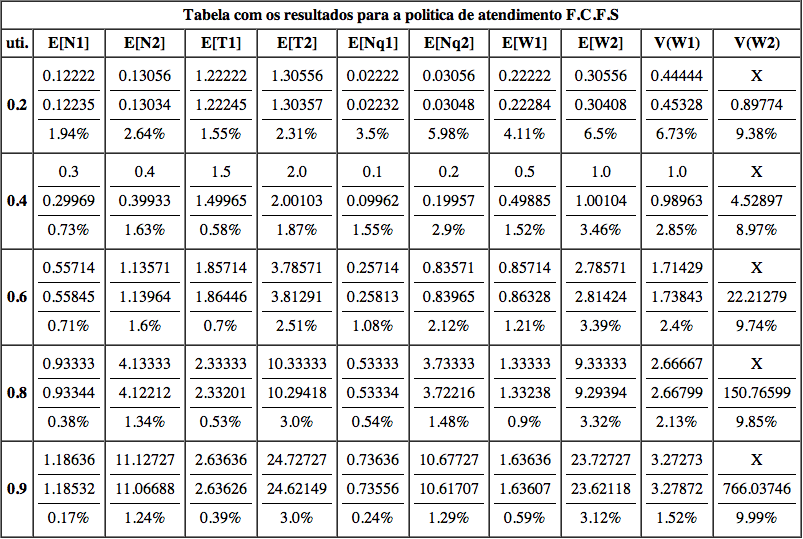
\includegraphics[width=1.0\textwidth]{tabelaFCFS.png}
   \caption{Tabela com os valores para a política de atendimento First Come First Served.}
\end{figure}

\pagebreak
\begin{figure}[htb!]
   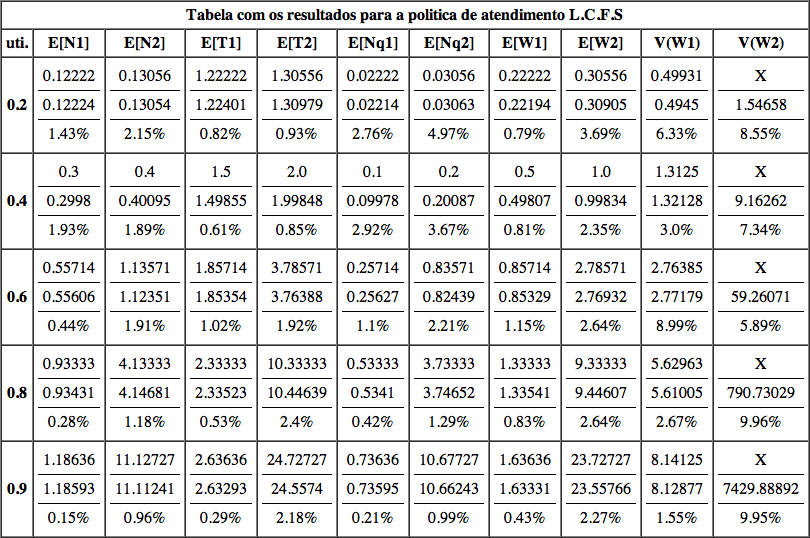
\includegraphics[width=1.0\textwidth]{tabelaLCFS.png}
   \caption{Tabela com os valores para a política de atendimento Last Come First Served.}
\end{figure}

\pagebreak

\section{Comentários}
\label{sec:coment}
aqui começa a seção comentários

\chapter{Otimização}

O fator mínimo que satisfaz a validação do intervalo de confiança para todos os valores de utilização é o mesmo que satisfaz o caso mais crítico, ou seja, com o sistema com valor de utilização igual a 0,9.

Como o método utilizado para a simulação foi o replicativo, o tamanho da fase transiente é considerado em cada rodada do simulador.

\section{Fatores mínimos}
\label{sec:fatores}

O valor calculado para os fatores mínimos de cada política são mostrados a seguir:\\

\textbf{F.C.F.S (First Come First Served):}
\begin{itemize}
  \item FATOR MÍNIMO $= (\# rodadas) * (tamanho da rodada + fases transientes)$
  \item FATOR MÍNIMO $= 76 * (100.000 + 500.000)$
  \item FATOR MÍNIMO $= 45.600.000$
\end{itemize}

\textbf{L.C.F.S (Last Come First Served):}
\begin{itemize}
  \item FATOR MÍNIMO $= (\# rodadas) * (tamanho da rodada + fases transientes)$
  \item FATOR MÍNIMO $= 106 * (100.000 + 500.000)$
  \item FATOR MÍNIMO $= 63.600.000$
\end{itemize}

\chapter{Conclusões}

Inicialmente encontramos dificuldades em implementar a lógica do simulador em si. Seguindo as instruções do capítulo de simulação da apostila, conseguimos ter uma ideia razoável das estruturas de dados necessárias e do fluxo desses dados pelo simulador para que ele gere os resultados corretos. Por exemplo, a lista de eventos, a estrutura de cada evento e o modo com que esses eventos são tratados e gerados pelo simulador são implementados da mesma forma que é explicada na apostila.

A forma como implementamos a lista de eventos do simulador mudou duas vezes durante a codificação do trabalho, já que encontramos dificuldades em encontrar a forma mais adequada em termos de perfomance para criar e gerenciar essa lista. Tendo em vista que ela é a estrutura mais importante do simulador, onde a maior parte do processamento é feito em cima dela, vimos como necessidade essencial otimiza-la da melhor maneira possível.

O uso da linguagem python facilitou bastante a implementação dos cálculos estatísticos do simulador, utilizando módulos como o scipy para o cálculo do valor da distribuição t de student para qualquer número de amostras. Esta facilidade pode ser comprovada analisando o tamanho dos métodos usados para o cálculo das médias, variâncias e intervalos de confiança dos módulos utilitários. O gerador de números aleatórios do python também facilitou bastante a implementação, pois, como é explicado na seção \ref{sec:random}, não foi necessário se preocupar com o valor da semente do gerador a cada rodada do método replicativo.

A geração dos gráficos necessários para a estimativa da fase transiente também foi feita sem menores dificuldades, devido ao uso da linguagem python.

Usamos o módulo psyco para agilizar a execução do programa. 

A implementação desse simulador aumentou significativamente o nosso entendimento sobre o sistema de rede de filas, foi possível verificar na prática as diferenças entre um sistema transiente e em equilíbrio; a evolução de um cliente dentro do sistema; o fato de que as médias são iguais para as duas políticas de atendimento, porém as variâncias são bastante distintas; e que os valores calculados de forma analítica puderam ser comprovados executando o simulador para todos os casos.

\chapter{Implementação}
Anexo - Listagem documentada do programa
A documentação do programa fonte deverá ser feita com rigor, explicando cada sub-rotina
ou passo da programação. Código fonte sem comentários não é aceitável. Mande a listagem
do código fonte como um anexo ao relatório. Uma versão eletrônica do documento
impresso deve ser disponibilizada.
O Grupo deve apresentar um executável funcionando em PC Windows ou Linux Ubuntu.
O relatório completo deve ser entregue impresso (e não em mídia eletrônica).
O programa executável deverá ser enviado para aguiar@nce.ufrj.br.
Se o Grupo usar alguma linguagem específica, ele deve compilar o ambiente e apresentar
um executável que rode sem necessidade de instalação especial, em Windows 7 ou Ubuntu.
O programa será testado com alguns valores particulares para averiguar sua correção e
integridade.



\end{document}
